\documentclass[12pt]{scrreprt}

%\documentclass[a4paper, 12pt, oneside]{scrbook}

%Eingaben

\usepackage[latin1, utf8]{inputenc}

\usepackage[T1]{fontenc}

\usepackage[ngermanb, english]{babel}

\usepackage{amsmath}
\usepackage{amsthm}
\usepackage{ulem}
%Layout

\usepackage{lmodern}

\usepackage{hyperref}

\usepackage[all]{hypcap} %Bei Verlinkungen auf Bilder die obere Grenze des Bildes verkinken.

%Für die Erzeugung von Graphiken

\usepackage{tikz}

%\usepackage{graphicx}

%Quellcode

\usepackage{listings}
\usepackage{graphicx}
\usepackage{color}

\lstdefinestyle{Shell}{delim=[il][\bfseries]{BB}}

\lstset{flexiblecolumns = true}

%

\usepackage[verbose]{placeins}

\usepackage{float} % for option H

% code highlighting

\usepackage{listings}
\usepackage{color}
 
\definecolor{codegreen}{rgb}{0,0.6,0}
\definecolor{codegray}{rgb}{0.5,0.5,0.5}
\definecolor{codepurple}{rgb}{0.58,0,0.82}
\definecolor{backcolour}{rgb}{0.95,0.95,0.92}
 
\lstdefinestyle{mystyle}{
    backgroundcolor=\color{backcolour},   
    commentstyle=\color{codegreen},
    keywordstyle=\color{magenta},
    numberstyle=\tiny\color{codegray},
    stringstyle=\color{codepurple},
    basicstyle=\footnotesize,
    breakatwhitespace=false,         
    breaklines=true,                 
    captionpos=b,                    
    keepspaces=true,                 
    numbers=left,                    
    numbersep=5pt,                  
    showspaces=false,                
    showstringspaces=false,
    showtabs=false,                  
    tabsize=2
}
 
\lstset{style=mystyle}


%\usepackage{siunitx}%schreibt einheiten richtig mit gutem abstand und richtige schriftzeichen
%\[v=\SI{2.3}{\metre\per\second}]
%\sisetup{% DE macht komma;
%  locale = UK%,
  %group-separator = {.} %,
  %per-mode = symbol
%}klappt irgendwie nicht so wie es soll


    \usepackage{xcolor} % Allow colors to be defined
    \usepackage{upquote} % Upright quotes for verbatim code
    \usepackage{fancyvrb} % verbatim replacement that allows latex
    \newcommand{\VerbatimStringTok}[1]{\textcolor[rgb]{0.25,0.44,0.63}{{#1}}}


\usepackage[scaled]{beramono}

\lstset{
  language=Python
}
\usepackage{enumitem}


    % Exact colors from NB
    \definecolor{incolor}{rgb}{0.0, 0.0, 0.5}
    \definecolor{outcolor}{rgb}{0.545, 0.0, 0.0}

    \DefineVerbatimEnvironment{Highlighting}{Verbatim}{commandchars=\\\{\}}


\begin{document}
%\titlehead{}
\subject{Data Science}
\title{Documentation}
\subtitle{Regression-Primer}
\author{}
\date{\large{\today}}
\publishers{Eicker Niklas, Halastra Szymon}
%\extratitle{\centering Schmutztitel}
%\uppertitleback{Obiger Titelrückentitel}
%\lowertitleback{Unterer Rückseitentitel}
%\dedication{Rückseite der Titelseite}
\maketitle
\tableofcontents



\chapter{Introduction} 
\label{chpt:intro}

For the following tasks we will use Graphlab and Numpy to read and analize data about sold houses. With several different models we will predict prices or other features of houses.

\section{Tasks}
\label{sec:task}

\begin{itemize}
\item Load house sales data: kc\_house\_data.csv.zip
\item What is the content, could you read it? do you understand collumns?
\item Explore the data for housing
\begin{itemize}
  \item make scatter plot of selected features
  \item create simple regression model of sqft\_living to price
  \item evaluate a simple model
  \item is linear function good enough? try quadratic polynomial  
\end{itemize}

\item Split your data into training sample and test sample
\begin{itemize}
  \item what is trainign error and testing error of your model?
  \item predict the house price for a given sqft\_living
  \item predict the sqft\_living for a given price of the house
  \item add more feaures
  \item is the model better now?
  \item maybe using range of data would work better?
  \item predict house price for a house id = 5309101299
      what is this house like?
  \item predict house price for a house id = 1925069082  
\end{itemize}
\end{itemize}

\section{Dataset}
\label{sec:data}

We have 21613 rows of the following data given in the dataset: 

\begin{center}
  \begin{tabular}{| c | c |}
    \hline
    \textbf{Feature} & \textbf{Type}\\
    \hline
    \hline
    id & int \\ \hline
    date & str \\ \hline
    price & float \\ \hline
    bedrooms & int \\ \hline
    bathrooms & float \\ \hline
    sqft\_living & int \\ \hline
    sqft\_lot & int \\ \hline
    floors & float \\ \hline
    waterfront & int \\ \hline
    view & int \\ \hline
    condition & int \\ \hline
    grade & int \\ \hline
    sqft\_above & int \\ \hline
    sqft\_basement & int \\ \hline
    yr\_built & int \\ \hline
    yr\_renovated & int \\ \hline
    zipcode & int \\ \hline
    lat & float \\ \hline
    long & float \\ \hline
    sqft\_living15 & int \\ \hline
    sqft\_lot15 & int \\ \hline
    const & float \\ \hline
    sqft\_living\_sq & float \\ \hline
  \end{tabular}
\end{center}

The houses are in Seattle, as can be seen with the zipcodes and were sold between 2014 and 2015, thus the data is quite new.\\


\chapter{Simple regression models} 
\label{chpt:srm}

\noindent
For the beginning we concentrated on the features \textit{price} and \textit{sqft\_living}. The distribution of these two features can be seen in figure \ref{fig:scatter}.\\

\begin{figure}[H]
\begin{center}
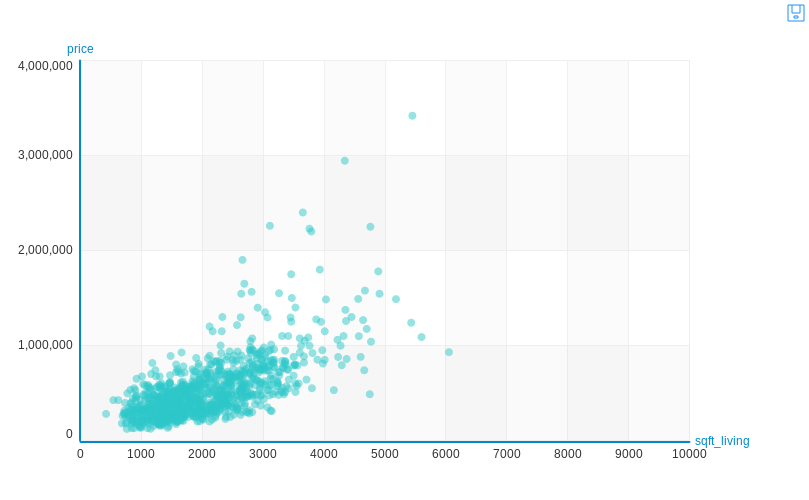
\includegraphics[width=0.9\textwidth, angle=0]{scatter_sqft_living_price.png}
\caption{Scatter plot of the two features \textit{price} and \textit{sqft\_living}.}
\label{fig:scatter}
\end{center}
\end{figure}

\section{Linear and quadratic model} 

As a first model we created a linear model with the target 'price' and fitted on a constant feature and 'sqft\_living'. As one can see in the scatter plot \ref{fig:scatter} the distribution around a single, straight line will be quite broad, which we will see in the RMS.\\

To compare with the linear fit, we also created a quadratic fit with a constant feature, 'sqft\_living' and squared 'sqft\_living'. The squared squarefoot-living values were saved in an additional column of our data.\\

The evaluation of both does not show a significant improvement of the quadratic fit over the linear fit. The RMS improves from 261440 to 250948 as can be seen in the table \ref{tab:rmse_models}.\\

\begin{table}[H]
  \caption{Comparison of the RMS of the linear and quadratic model}
  \label{tab:rmse_models}
  \begin{center}
    \begin{tabular}{| c | c | c |}
      \hline
      & \textbf{Linear model} & \textbf{Quadratic model}\\
      \hline
      \hline
      \textbf{RMS} & 261441 & 250948 \\ \hline
      \textbf{max. Error} & 4362075 & 5913021 \\ \hline
    \end{tabular}	
  \end{center}
\end{table}

\chapter{Improved regression models} 
\label{chpt:irm}

\section{Training and testing sample}

The dataset is split up into a training sample and a testing sample. Randomly 80\% of the data is placed in the training sample, the other 20\% will be used to evaluate the model.\\

We created another linear model, but this time only on the training sample. The evaluation on the testing sample shows the same uncertainty as before, wich is what we expected for randomly picking the house data.\\

\begin{center}
\setitemize{wide}
	\begin{itemize}
		\item[RMS testing sample:] 255191
		\item[RMS training sample:] 262943
		\item[RMS whole data:] 261441
	\end{itemize}
\end{center}

\section{Predictions}

To predict prices with given square foot values and the other way arround, we define two methods:\\

\begin{lstlisting}
def get_house_price(sqft_living):
    return (sqft_model_lin.get('coefficients')['value'][0] + sqft_model_lin.get('coefficients')['value'][1] * sqft_living)
\end{lstlisting}

\begin{lstlisting}
def get_house_sqft(price):
    coeff = [sqft_model_lin.get('coefficients')['value'][1], (sqft_model_lin.get('coefficients')['value'][0] - price)]
    return np.roots(coeff)[0]
\end{lstlisting}

\vspace{0.5cm}
With these two methods some test values are calculated, which can be seen in tables \ref{tab:predict_sqft} and \ref{tab:predict_price}. The values are in the expected range and can be well compared with the scatter plot in chaper one \ref{fig:scatter}.\\


\begin{table}[H]
  \caption{Prediction of square feet living}
  \label{tab:predict_sqft}
\begin{center}
  \begin{tabular}{| c | c |}
    \hline
    \textbf{Given price} & \textbf{Predicted square foot living}\\
    \hline
    \hline
    500000 & 1940 \\ \hline
    1000000 & 3714 \\ \hline
    1500000 & 5487 \\ \hline
    2500000 & 9034 \\ \hline
  \end{tabular}
\end{center}
\end{table}

\begin{table}[H]
  \caption{Prediction of prices}
  \label{tab:predict_price}
\begin{center}
  \begin{tabular}{| c | c |}
    \hline
    \textbf{Given square foot living} & \textbf{Predicted price}\\
    \hline
    \hline
    1000 & 234844 \\ \hline
    2000 & 516802 \\ \hline
    3000 & 798760 \\ \hline
    4000 & 1080717 \\ \hline
  \end{tabular}
\end{center}
\end{table}

\section{Multi-feature model}
\label{sec:multi}

In a new model we include additional features: 'sqft\_living', 'sqft\_lot', 'grade', 'yr\_built'\\

The RMS goes down a bit to 232201, thus more features made the predictions more precise. To further improve on this we will eliminate outstanding houses from the data. From now on only data is used of houses with prices below $2000000$ and square foot living below $5000$.\\

The multi-feature model with the selected data has an RMS of 177179 on the testing samples. Meaning the RMS went down a considerable amount.\\

\section{Selective houses}
In the following we looked a bit closer at two selected houses.\\

\subsection{House nr. 2008000270}
The asked for house with the id 5309101299 does not exist. This is why we randomly chose another house from the data to take a closer look at.\\

The house with the ID 2008000270 is a rather small house, with 1060 sqft living and only one floor. The price is one of the lowest of the dataset with only 291850 dollar. There are 3 bedrooms and 1.5(?!) bathrooms. It was build in 1963.\\

\subsection{Prediciton for house nr. 1925069082}

The house number 1925069082 is worth more then 2 million and thus one of the data points that are far away from most of the others. It is even so far out of the bulk of data, that we cut it out of our dataset in section \ref{sec:multi}. The prediction with our model fails, as can be seen in table \ref{tab:predict_fail}.\\

\begin{table}[H]
  \caption{Prediction and data for house with id 1925069082}
  \label{tab:predict_fail}
\begin{center}
  \begin{tabular}{| c | c |}
    \hline
    \textbf{Predicted price} & \textbf{Real price}\\
    \hline
    \hline
    1261170 & 2200000 \\ \hline
  \end{tabular}
\end{center}
\end{table}


\end{document}